\documentclass{article}

% Hier befinden sich Pakete, die wir beinahe immer benutzen ...

\usepackage[utf8]{inputenc}

% Sprach-Paket:
\usepackage[ngerman]{babel}

% damit's nicht so, wie beim Grill aussieht:
\usepackage{fullpage}

% Mathematik:
\usepackage{amsmath, amssymb, amsfonts, amsthm}
\usepackage{bbm}
\usepackage{mathtools, mathdots}

% Makros mit mehereren Default-Argumenten:
\usepackage{twoopt}

% Anführungszeichen (Makro \Quote{}):
\usepackage{babel}

% if's für Makros:
\usepackage{xifthen}
\usepackage{etoolbox}

% tikz ist kein Zeichenprogramm (doch!):
\usepackage{tikz}

% bessere Aufzählungen:
\usepackage{enumitem}

% (bessere) Umgebung für Bilder:
\usepackage{graphicx, subfig, float}

% Umgebung für Code:
\usepackage{listings}

% Farben:
\usepackage{xcolor}

% Umgebung für "plain text":
\usepackage{verbatim}

% Umgebung für mehrerer Spalten:
\usepackage{multicol}

% "nette" Brüche
\usepackage{nicefrac}

% Spaltentypen verschiedener Dicke
\usepackage{tabularx}
\usepackage{makecell}

% Für Vektoren
\usepackage{esvect}

% (Web-)Links
\usepackage{hyperref}

% Zitieren & Literatur-Verzeichnis
\usepackage[style = authoryear]{biblatex}
\usepackage{csquotes}

% so ähnlich wie mathbb
%\usepackage{mathds}

% Keine Ahnung, was das macht ...
\usepackage{booktabs}
\usepackage{ngerman}
\usepackage{placeins}


\def \lastexercisenumber {15}

% special letters:

\newcommand{\N}{\mathbb{N}}
\newcommand{\Z}{\mathbb{Z}}
\newcommand{\Q}{\mathbb{Q}}
\newcommand{\R}{\mathbb{R}}
\newcommand{\C}{\mathbb{C}}
\newcommand{\K}{\mathbb{K}}
\newcommand{\T}{\mathbb{T}}
\newcommand{\E}{\mathbb{E}}
\newcommand{\V}{\mathbb{V}}
\renewcommand{\S}{\mathbb{S}}
\renewcommand{\P}{\mathbb{P}}
\newcommand{\1}{\mathbbm{1}}

% quantors:

\newcommand{\Forall}{\forall \,}
\newcommand{\Exists}{\exists \,}
\newcommand{\ExistsOnlyOne}{\exists! \,}
\newcommand{\nExists}{\nexists \,}
\newcommand{\ForAlmostAll}{\forall^\infty \,}

% MISC symbols:

\newcommand{\landau}{{\scriptstyle \mathcal{O}}}
\newcommand{\Landau}{\mathcal{O}}


\newcommand{\eps}{\mathrm{eps}}

% graphics in a box:

\newcommandtwoopt
{\includegraphicsboxed}[3][][]
{
  \begin{figure}[!h]
    \begin{boxedin}
      \ifthenelse{\isempty{#1}}
      {
        \begin{center}
          \includegraphics[width = 0.75 \textwidth]{#3}
          \label{fig:#2}
        \end{center}
      }{
        \begin{center}
          \includegraphics[width = 0.75 \textwidth]{#3}
          \caption{#1}
          \label{fig:#2}
        \end{center}
      }
    \end{boxedin}
  \end{figure}
}

% braces:

\newcommand{\pbraces}[1]{{\left  ( #1 \right  )}}
\newcommand{\bbraces}[1]{{\left  [ #1 \right  ]}}
\newcommand{\Bbraces}[1]{{\left \{ #1 \right \}}}
\newcommand{\vbraces}[1]{{\left  | #1 \right  |}}
\newcommand{\Vbraces}[1]{{\left \| #1 \right \|}}
\newcommand{\abraces}[1]{{\left \langle #1 \right \rangle}}
\newcommand{\round}[1]{\bbraces{#1}}

\newcommand
{\floorbraces}[1]
{{\left \lfloor #1 \right \rfloor}}

\newcommand
{\ceilbraces} [1]
{{\left \lceil  #1 \right \rceil }}

% special functions:

\newcommand{\norm}  [2][]{\Vbraces{#2}_{#1}}
\newcommand{\diam}  [2][]{\mathrm{diam}_{#1} \: #2}
\newcommand{\diag}  [1]{\mathrm{diag} \: #1}
\newcommand{\dist}  [1]{\mathrm{dist} \: #1}
\newcommand{\mean}  [1]{\mathrm{mean} \: #1}
\newcommand{\erf}   [1]{\mathrm{erf} \: #1}
\newcommand{\id}    [1]{\mathrm{id} \: #1}
\newcommand{\sgn}   [1]{\mathrm{sgn} \: #1}
\newcommand{\supp}  [1]{\mathrm{supp} \: #1}
\newcommand{\arsinh}[1]{\mathrm{arsinh} \: #1}
\newcommand{\arcosh}[1]{\mathrm{arcosh} \: #1}
\newcommand{\artanh}[1]{\mathrm{artanh} \: #1}
\newcommand{\card}  [1]{\mathrm{card} \: #1}
\newcommand{\Span}  [1]{\mathrm{span} \: #1}
\newcommand{\Aut}   [1]{\mathrm{Aut} \: #1}
\newcommand{\End}   [1]{\mathrm{End} \: #1}
\newcommand{\ggT}   [1]{\mathrm{ggT} \: #1}
\newcommand{\kgV}   [1]{\mathrm{kgV} \: #1}
\newcommand{\ord}   [1]{\mathrm{ord} \: #1}
\newcommand{\grad}  [1]{\mathrm{grad} \: #1}
\newcommand{\ran}   [1]{\mathrm{ran} \: #1}
\newcommand{\graph} [1]{\mathrm{graph} \: #1}
\newcommand{\Inv}   [1]{\mathrm{Inv} \: #1}
\newcommand{\pv}    [1]{\mathrm{pv} \: #1}
\newcommand{\GL}    [1]{\mathrm{GL} \: #1}
\newcommand{\Mod}{\mathrm{Mod} \:}
\newcommand{\Th}{\mathrm{Th} \:}
\newcommand{\Char}{\mathrm{char}}
\newcommand{\At}{\mathrm{At}}
\newcommand{\Ob}{\mathrm{Ob}}
\newcommand{\Hom}{\mathrm{Hom}}
\newcommand{\orthogonal}[3][]{#2 ~\bot_{#1}~ #3}
\newcommand{\Rang}{\mathrm{Rang}}
\newcommand{\NIL}{\mathrm{NIL}}
\newcommand{\Res}{\mathrm{Res}}
\newcommand{\lxor}{\dot \lor}
\newcommand{\Div}{\mathrm{div} \:}
\newcommand{\meas}{\mathrm{meas} \:}

% fractions:

\newcommand{\Frac}[2]{\frac{1}{#1} \pbraces{#2}}
\newcommand{\nfrac}[2]{\nicefrac{#1}{#2}}

% derivatives & integrals:

\newcommandtwoopt
{\Int}[4][][]
{\int_{#1}^{#2} #3 ~\mathrm{d} #4}

\newcommandtwoopt
{\derivative}[3][][]
{
  \frac
  {\mathrm{d}^{#1} #2}
  {\mathrm{d} #3^{#1}}
}

\newcommandtwoopt
{\pderivative}[3][][]
{
  \frac
  {\partial^{#1} #2}
  {\partial #3^{#1}}
}

\newcommand
{\primeprime}
{{\prime \prime}}

\newcommand
{\primeprimeprime}
{{\prime \prime \prime}}

% Text:

\newcommand{\Quote}[1]{\glqq #1\grqq{}}
\newcommand{\Text}[1]{{\text{#1}}}
\newcommand{\fastueberall}{\text{f.ü.}}
\newcommand{\fastsicher}{\text{f.s.}}

% -------------------------------- %
% amsthm-stuff:

\theoremstyle{definition}

% numbered theorems
\newtheorem{theorem}{Satz}
\newtheorem{lemma}{Lemma}
\newtheorem{corollary}{Korollar}
\newtheorem{proposition}{Proposition}
\newtheorem{remark}{Bemerkung}
\newtheorem{definition}{Definition}
\newtheorem{example}{Beispiel}

% unnumbered theorems
\newtheorem*{theorem*}{Satz}
\newtheorem*{lemma*}{Lemma}
\newtheorem*{corollary*}{Korollar}
\newtheorem*{proposition*}{Proposition}
\newtheorem*{remark*}{Bemerkung}
\newtheorem*{definition*}{Definition}
\newtheorem*{example*}{Beispiel}

% Please define this stuff in project ("main.tex"):

% \def \lastexercisenumber {...}
% This will be 0 by default

% \setcounter{section}{...}
% This will be 0 by default
% and hence, completely ignored

\ifnum \thesection = 0
{\newtheorem{exercise}{Aufgabe}}
\else
{\newtheorem{exercise}{Aufgabe}[section]}
\fi

\ifdef
{\lastexercisenumber}
{\setcounter{exercise}{\lastexercisenumber}}

\newcommand{\solution}
{
    \renewcommand{\proofname}{Lösung}
    \renewcommand{\qedsymbol}{}
    \proof
}

\renewcommand{\proofname}{Beweis}

% -------------------------------- %
% environment zum einkasteln:

% dickere vertical lines
\newcolumntype
{x}
[1]
{!{\centering\arraybackslash\vrule width #1}}

% environment selbst (the big cheese)
\newenvironment
{boxedin}
{
  \begin{tabular}
  {
    x{1 pt}
    p{\textwidth}
    x{1 pt}
  }
  \Xhline
  {2 \arrayrulewidth}
}
{
  \\
  \Xhline{2 \arrayrulewidth}
  \end{tabular}
}

% -------------------------------- %
% MISC "Ein-Deutschungen"

\renewcommand
{\figurename}
{Abbildung}

\renewcommand
{\tablename}
{Tabelle}

% -------------------------------- %

% ---------------------------------------------------------------- %
% https://www.overleaf.com/learn/latex/Code_listing

\definecolor{codegreen} {rgb}{0, 0.6, 0}
\definecolor{codegray}    {rgb}{0.5, 0.5, 0.5}
\definecolor{codepurple}{rgb}{0.58, 0, 0.82}
\definecolor{backcolour}{rgb}{0.95, 0.95, 0.92}

\lstdefinestyle{overleaf}
{
    backgroundcolor = \color{backcolour},
    commentstyle = \color{codegreen},
    keywordstyle = \color{magenta},
    numberstyle = \tiny\color{codegray},
    stringstyle = \color{codepurple},
    basicstyle = \ttfamily \footnotesize,
    breakatwhitespace = false,
    breaklines = true,
    captionpos = b,
    keepspaces = true,
    numbers = left,
    numbersep = 5pt,
    showspaces = false,
    showstringspaces = false,
    showtabs = false,
    tabsize = 2
}

% ---------------------------------------------------------------- %
% https://en.wikibooks.org/wiki/LaTeX/Source_Code_Listings

\lstdefinestyle{customc}
{
    belowcaptionskip = 1 \baselineskip,
    breaklines = true,
    frame = L,
    xleftmargin = \parindent,
    language = C,
    showstringspaces = false,
    basicstyle = \footnotesize \ttfamily,
    keywordstyle = \bfseries \color{green!40!black},
    commentstyle = \itshape \color{purple!40!black},
    identifierstyle = \color{blue},
    stringstyle = \color{orange},
}

\lstdefinestyle{customasm}
{
    belowcaptionskip = 1 \baselineskip,
    frame = L,
    xleftmargin = \parindent,
    language = [x86masm] Assembler,
    basicstyle = \footnotesize\ttfamily,
    commentstyle = \itshape\color{purple!40!black},
}

% ---------------------------------------------------------------- %
% https://tex.stackexchange.com/questions/235731/listings-syntax-for-literate

\definecolor{maroon}        {cmyk}{0, 0.87, 0.68, 0.32}
\definecolor{halfgray}      {gray}{0.55}
\definecolor{ipython_frame} {RGB}{207, 207, 207}
\definecolor{ipython_bg}    {RGB}{247, 247, 247}
\definecolor{ipython_red}   {RGB}{186, 33, 33}
\definecolor{ipython_green} {RGB}{0, 128, 0}
\definecolor{ipython_cyan}  {RGB}{64, 128, 128}
\definecolor{ipython_purple}{RGB}{170, 34, 255}

\lstdefinestyle{stackexchangePython}
{
    breaklines = true,
    %
    extendedchars = true,
    literate =
    {á}{{\' a}} 1 {é}{{\' e}} 1 {í}{{\' i}} 1 {ó}{{\' o}} 1 {ú}{{\' u}} 1
    {Á}{{\' A}} 1 {É}{{\' E}} 1 {Í}{{\' I}} 1 {Ó}{{\' O}} 1 {Ú}{{\' U}} 1
    {à}{{\` a}} 1 {è}{{\` e}} 1 {ì}{{\` i}} 1 {ò}{{\` o}} 1 {ù}{{\` u}} 1
    {À}{{\` A}} 1 {È}{{\' E}} 1 {Ì}{{\` I}} 1 {Ò}{{\` O}} 1 {Ù}{{\` U}} 1
    {ä}{{\" a}} 1 {ë}{{\" e}} 1 {ï}{{\" i}} 1 {ö}{{\" o}} 1 {ü}{{\" u}} 1
    {Ä}{{\" A}} 1 {Ë}{{\" E}} 1 {Ï}{{\" I}} 1 {Ö}{{\" O}} 1 {Ü}{{\" U}} 1
    {â}{{\^ a}} 1 {ê}{{\^ e}} 1 {î}{{\^ i}} 1 {ô}{{\^ o}} 1 {û}{{\^ u}} 1
    {Â}{{\^ A}} 1 {Ê}{{\^ E}} 1 {Î}{{\^ I}} 1 {Ô}{{\^ O}} 1 {Û}{{\^ U}} 1
    {œ}{{\oe}}  1 {Œ}{{\OE}}  1 {æ}{{\ae}}  1 {Æ}{{\AE}}  1 {ß}{{\ss}}  1
    {ç}{{\c c}} 1 {Ç}{{\c C}} 1 {ø}{{\o}} 1 {å}{{\r a}} 1 {Å}{{\r A}} 1
    {€}{{\EUR}} 1 {£}{{\pounds}} 1
}


% Python definition (c) 1998 Michael Weber
% Additional definitions (2013) Alexis Dimitriadis
% modified by me (should not have empty lines)

\lstdefinelanguage{iPython}{
    morekeywords = {access, and, break, class, continue, def, del, elif, else, except, exec, finally, for, from, global, if, import, in, is, lambda, not, or, pass, print, raise, return, try, while}, %
    %
    % Built-ins
    morekeywords = [2]{abs, all, any, basestring, bin, bool, bytearray, callable, chr, classmethod, cmp, compile, complex, delattr, dict, dir, divmod, enumerate, eval, execfile, file, filter, float, format, frozenset, getattr, globals, hasattr, hash, help, hex, id, input, int, isinstance, issubclass, iter, len, list, locals, long, map, max, memoryview, min, next, object, oct, open, ord, pow, property, range, raw_input, reduce, reload, repr, reversed, round, set, setattr, slice, sorted, staticmethod, str, sum, super, tuple, type, unichr, unicode, vars, xrange, zip, apply, buffer, coerce, intern}, %
    %
    sensitive = true, %
    morecomment = [l] \#, %
    morestring = [b]', %
    morestring = [b]", %
    %
    morestring = [s]{'''}{'''}, % used for documentation text (mulitiline strings)
    morestring = [s]{"""}{"""}, % added by Philipp Matthias Hahn
    %
    morestring = [s]{r'}{'},     % `raw' strings
    morestring = [s]{r"}{"},     %
    morestring = [s]{r'''}{'''}, %
    morestring = [s]{r"""}{"""}, %
    morestring = [s]{u'}{'},     % unicode strings
    morestring = [s]{u"}{"},     %
    morestring = [s]{u'''}{'''}, %
    morestring = [s]{u"""}{"""}, %
    %
    % {replace}{replacement}{lenght of replace}
    % *{-}{-}{1} will not replace in comments and so on
    literate = 
    {á}{{\' a}} 1 {é}{{\' e}} 1 {í}{{\' i}} 1 {ó}{{\' o}} 1 {ú}{{\' u}} 1
    {Á}{{\' A}} 1 {É}{{\' E}} 1 {Í}{{\' I}} 1 {Ó}{{\' O}} 1 {Ú}{{\' U}} 1
    {à}{{\` a}} 1 {è}{{\` e}} 1 {ì}{{\` i}} 1 {ò}{{\` o}} 1 {ù}{{\` u}} 1
    {À}{{\` A}} 1 {È}{{\' E}} 1 {Ì}{{\` I}} 1 {Ò}{{\` O}} 1 {Ù}{{\` U}} 1
    {ä}{{\" a}} 1 {ë}{{\" e}} 1 {ï}{{\" i}} 1 {ö}{{\" o}} 1 {ü}{{\" u}} 1
    {Ä}{{\" A}} 1 {Ë}{{\" E}} 1 {Ï}{{\" I}} 1 {Ö}{{\" O}} 1 {Ü}{{\" U}} 1
    {â}{{\^ a}} 1 {ê}{{\^ e}} 1 {î}{{\^ i}} 1 {ô}{{\^ o}} 1 {û}{{\^ u}} 1
    {Â}{{\^ A}} 1 {Ê}{{\^ E}} 1 {Î}{{\^ I}} 1 {Ô}{{\^ O}} 1 {Û}{{\^ U}} 1
    {œ}{{\oe}}  1 {Œ}{{\OE}}  1 {æ}{{\ae}}  1 {Æ}{{\AE}}  1 {ß}{{\ss}}  1
    {ç}{{\c c}} 1 {Ç}{{\c C}} 1 {ø}{{\o}} 1 {å}{{\r a}} 1 {Å}{{\r A}} 1
    {€}{{\EUR}} 1 {£}{{\pounds}} 1
    %
    {^}{{{\color{ipython_purple}\^ {}}}} 1
    { = }{{{\color{ipython_purple} = }}} 1
    %
    {+}{{{\color{ipython_purple}+}}} 1
    {*}{{{\color{ipython_purple}$^\ast$}}} 1
    {/}{{{\color{ipython_purple}/}}} 1
    %
    {+=}{{{+=}}} 1
    {-=}{{{-=}}} 1
    {*=}{{{$^\ast$ = }}} 1
    {/=}{{{/=}}} 1,
    literate = 
    *{-}{{{\color{ipython_purple} -}}} 1
     {?}{{{\color{ipython_purple} ?}}} 1,
    %
    identifierstyle = \color{black}\ttfamily,
    commentstyle = \color{ipython_cyan}\ttfamily,
    stringstyle = \color{ipython_red}\ttfamily,
    keepspaces = true,
    showspaces = false,
    showstringspaces = false,
    %
    rulecolor = \color{ipython_frame},
    frame = single,
    frameround = {t}{t}{t}{t},
    framexleftmargin = 6mm,
    numbers = left,
    numberstyle = \tiny\color{halfgray},
    %
    %
    backgroundcolor = \color{ipython_bg},
    % extendedchars = true,
    basicstyle = \scriptsize,
    keywordstyle = \color{ipython_green}\ttfamily,
}

% ---------------------------------------------------------------- %
% https://tex.stackexchange.com/questions/417884/colour-r-code-to-match-knitr-theme-using-listings-minted-or-other

\geometry{verbose, tmargin = 2.5cm, bmargin = 2.5cm, lmargin = 2.5cm, rmargin = 2.5cm}

\definecolor{backgroundCol}  {rgb}{.97, .97, .97}
\definecolor{commentstyleCol}{rgb}{0.678, 0.584, 0.686}
\definecolor{keywordstyleCol}{rgb}{0.737, 0.353, 0.396}
\definecolor{stringstyleCol} {rgb}{0.192, 0.494, 0.8}
\definecolor{NumCol}         {rgb}{0.686, 0.059, 0.569}
\definecolor{basicstyleCol}  {rgb}{0.345, 0.345, 0.345}

\lstdefinestyle{stackexchangeR}
{
    language = R,                                        % the language of the code
    basicstyle = \small \ttfamily \color{basicstyleCol}, % the size of the fonts that are used for the code
    % numbers = left,                                      % where to put the line-numbers
    numberstyle = \color{green},                         % the style that is used for the line-numbers
    stepnumber = 1,                                      % the step between two line-numbers. If it is 1, each line will be numbered
    numbersep = 5pt,                                     % how far the line-numbers are from the code
    backgroundcolor = \color{backgroundCol},             % choose the background color. You must add \usepackage{color}
    showspaces = false,                                  % show spaces adding particular underscores
    showstringspaces = false,                            % underline spaces within strings
    showtabs = false,                                    % show tabs within strings adding particular underscores
    % frame = single,                                      % adds a frame around the code
    % rulecolor = \color{white},                           % if not set, the frame-color may be changed on line-breaks within not-black text (e.g. commens (green here))
    tabsize = 2,                                         % sets default tabsize to 2 spaces
    captionpos = b,                                      % sets the caption-position to bottom
    breaklines = true,                                   % sets automatic line breaking
    breakatwhitespace = false,                           % sets if automatic breaks should only happen at whitespace
    keywordstyle = \color{keywordstyleCol},              % keyword style
    commentstyle = \color{commentstyleCol},              % comment style
    stringstyle = \color{stringstyleCol},                % string literal style
    literate = %
    *{0}{{{\color{NumCol} 0}}} 1
     {1}{{{\color{NumCol} 1}}} 1
     {2}{{{\color{NumCol} 2}}} 1
     {3}{{{\color{NumCol} 3}}} 1
     {4}{{{\color{NumCol} 4}}} 1
     {5}{{{\color{NumCol} 5}}} 1
     {6}{{{\color{NumCol} 6}}} 1
     {7}{{{\color{NumCol} 7}}} 1
     {8}{{{\color{NumCol} 8}}} 1
     {9}{{{\color{NumCol} 9}}} 1
}

% ---------------------------------------------------------------- %
% Fundament Mathematik

\lstdefinestyle{fundament}{basicstyle = \ttfamily}

% ---------------------------------------------------------------- %


\parskip 0pt
\parindent 0pt

\title
{
  Numerik von Differentialgleichungen - Übung 4 \\
  \vspace{4pt}
  \normalsize
  \textit{4. UE am 22.04.2020}
}
\author
{
  Richard Weiss       \and
  Florian Schager     \and
  Christian Sallinger \and
  Christian Göth
}
\date{}

\begin{document}

\maketitle

\begin{exercise}
Wenden Sie die Methode der (Zweischritt-)Richardson Extrapolation aus Abschnitt
2.7 auf das explizite Euler-Verfahren an.
\begin{itemize}
  \item [\textbf{a)}] Welches Verfahren entsteht dabei?
  \item [\textbf{b)}] Weisen Sie unabhängig von Abschnitt 2.7 nach, dass dieses
  Verfahren die Konvergenzordnung 2 besitzt.
\end{itemize}
\end{exercise}
\begin{solution}
\leavevmode \\
\begin{itemize}
  \item [\textbf{a)}] Explizites Euler-Verfahren: $\varphi(t,y,h) = f(t,y)$
  Für hinreichend glattes $f$ erhalten wir nach Taylor die asymptotische Entwicklung
  \begin{align*}
    z(t+h) = z(t) + hf(t,z(t),h) + \frac{h^2}{2}y^{\primeprime} + \Landau{h^3}
  \end{align*}
  Ergo können wir die Richardson-Extrapolation anwenden und erhalten damit
  \begin{align*}
    z_1 &:= z(t) + hf(t,z(t)) \\
    \widetilde{z}_{1/2} &= z(t) + \frac{h}{2}f(t,z(t)) \\
  \widetilde{z_1} &:= \widetilde{z}_{1/2} + \frac{h}{2}f(t + \frac{h}{2},\widetilde{z}_{1/2}) \\
  &= z(t) + \frac{h}{2}f(t,z(t)) + \frac{h}{2}f(t + \frac{h}{2},z(t) + \frac{h}{2}f(t,z(t))) \\
    z(t + h) &\approx 2\widetilde{z_1} - \widetilde{z_1}
    = 2z(t) + h\left(f(t,z(t))+ f(t+\frac{h}{2},z(t)+\frac{h}{2}f(t,z(t)))\right) -
    (z(t) + hf(t,z(t))) \\
    &= z(t) + hf(t+\frac{h}{2},z(t)+\frac{h}{2}f(t,z(t)))
  \end{align*}
  die modifizierte Eulermethode.
  \item [\textbf{b)}] Nach Proposition 2.17 hat das Einschrittverfahren der Form
  \begin{align*}
    \phi(t,y,h) := b_1f(t,y) + b_2f(t+ch,y+ahf(t,y))
  \end{align*}
  genau dann Konsistenzordnung 2, wenn $a = c$ $b_1 + b_2 = 1$ und $2b_2a = 1$. \\
  In unserem Fall haben wir $b_1 = 0, b_2 = 1, a = c = 1/2$ und die Bedingungen
  werden offensichtlich erfüllt.
\end{itemize}
\end{solution}

\begin{exercise}
Implementieren Sie das implizite Euler-Verfahren unter Verwendung des Newton-Verfahrens
zur Lösung des nichtlinearen Gleichungssystems. Der Algorithmus soll als Input-Parameter
einen Vektor von Stützstellen $t$, einen Startwert $y_0$, die rechte Seite und Ableitung
der rechten Seite $f$, beziehungsweise $\frac{\partial}{\partial y} f$, sowie eine
geeignete Abbruchbedingung für das Newton-Verfahren (Toleranz und/oder maximale
Anzahl an Iterationen) akzeptieren. \\
Testen Sie das Verfahren an folgenden Anfangswertproblemen: Sei $Y = (y_1,y_2)^{\top}$
die Lösung des Anfangswertproblems
\begin{align}
  Y^{\prime}(t) = \begin{pmatrix}
    -2 & 1 \\
    1 & -2
  \end{pmatrix}Y(t) +
  \begin{pmatrix}
    2 \sin(t) \\ 2(\cos(t) - \sin(t))
  \end{pmatrix},\quad t \geq 0, \qquad
  Y(0) = \begin{pmatrix}
    2 \\ 3
  \end{pmatrix}.
\end{align}
Sei $Z = (z_1,z_2)^{\top}$ die Lösung des Anfangswertproblems
\begin{align}
Z^{\prime}(t) = \begin{pmatrix}
  -2 & 1 \\ 998 & -999
\end{pmatrix}Z(t) +
\begin{pmatrix}
  2\sin(t) \\ 999(\cos(t)-\sin(t))
\end{pmatrix}, \quad t \geq 0, \qquad
Z(0) = \begin{pmatrix}
  2 \\ 3
\end{pmatrix}.
\end{align}
Vergleichen Sie dabei auch mit den Ergebnissen und Schrittweiten des eingebetteten
Runge-Kutta-Verfahren RK5(4) aus Aufgabe 15. Verwenden Sie dazu die Parameter $t \in
[0,10], \rho = 0.7, \eta = 1.5,$ tol$=10^{-6}, h_{\min} = 10^{-10}$.
\end{exercise}
\begin{solution}
Wir beobachten, dass beide Differentialgleichungen zu annähernd gleichen Ergebnissen
führen, im zweiten Fall werden allerdings im eingebetteten Runge-Kutta-Verfahren
deutlich kleinere Schrittweiten für die selbe Genauigkeit benötigt.
\FloatBarrier
\begin{figure}
    \centering
    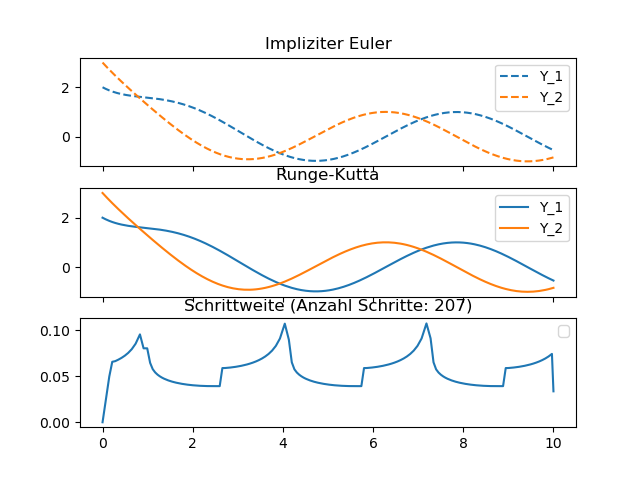
\includegraphics[width=\linewidth]{plot1_advanced.png}
    \caption{Y}
\end{figure}
\begin{figure}
    \centering
    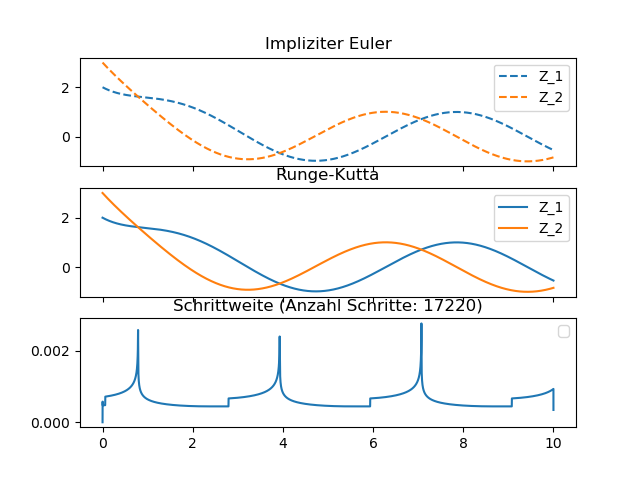
\includegraphics[width=\linewidth]{plot2_advanced.png}
    \caption{Z}
\end{figure}
\end{solution}

\FloatBarrier
\begin{exercise}
Gegeben sei ein implizites, $s$-stufiges Runge-Kutta-Verfahren der Form
\renewcommand{\arraystretch}{1.5}
\begin{align}
  \begin{matrix}
  c & \vline & A \\
  \hline
  0 & \vline & b^{\top}
  \end{matrix}.
\end{align}
Zeigen Sie: Angewendet auf das Anfangswertproblem $y^{\prime} = \lambda y$ mit
$y(0) = y_0$ und $\lambda \in \mathbb{C}$ gilt für hinreichend kleine $h$
\begin{align}
  y_{i+1} = R(\lambda h)y_i
\end{align}
mit einer rationalen Funktion $R = P/Q$ und Polynomen $P,Q \in \Pi_s$ vom
maximalen Grad $s$.
\end{exercise}
\begin{solution}
Beweis.
\end{solution}

\begin{exercise}
Beweisen Sie, welche Konsistenzordnungen diese impliziten Runge-Kutta-Verfahren besitzen.
\begin{itemize}
  \item (Example 3.11) Impliziter Euler
  \item (Example 3.12) Implizite Trapezregel
  \item (Example 3.13) Implizite Mittelpunktsregel
\end{itemize}
\end{exercise}
\begin{solution}
\leavevmode \\
\begin{itemize}
  \item Impliziter Euler:
  \begin{align*}
    y_{l+1} = y_l + h_lk_1 = y_l + hf(t_l+h_l,y_l+h_lk_1) = f(t_{l+1},y_{l+1})
  \end{align*}
  Mit dem Satz von Taylor folgt für hinreichend glattes f
  \begin{align*}
    y(t) = y(t+h) - hy^{\prime}(t+h) + \Landau{h^2} =
    y(t+h) - hf(t+h,y(t+h)) + \Landau{h^2}
  \end{align*}
  und damit
  \begin{align*}
    \tau(t,y,h) = ||y(t+h) - y(t) - h\phi(t,y(t),h)|| =
    ||y(t+h) - y(t) - hf(t + h,y(t+h))|| \leq Ch^2.
  \end{align*}
  Also hat das implizite Euler-Verfahren Konsistenzordnung 1.
  \item Implizite Trapezregel:
  \begin{align*}
    y_{l+1} = y_l + h_l\frac{f(t_l,y_l) + f(t_{l+1},y_{l+1})}{2}
  \end{align*}
  \begin{align*}
    \tau(t,y,h) = ||y(t+h) - y(t) - h\phi(t,y(t),h)|| =
    ||y(t+h) - y(t) - \frac{h}{2}\left(f(t,y) + f(t+h,y+h)\right)||
  \end{align*}
  Wir kennen die Restglieddarstellung der Trapezregel:
  \begin{align*}
    Q(f) - \frac{b-a}{2}(f(a)+f(b)) = -\frac{(b-a)^3}{12}f^{\primeprime}(\xi)
  \end{align*}
  Damit erhalten wir
  \begin{align*}
  \left\|y(t+h) - y(t) - \frac{h}{2}\left(f(t,y) + f(t+h,y+h)\right)\right\|
  &= \left\|\int_{t}^{t+h}f(\tau,y(\tau))d\tau - \frac{h}{2}\left(f(t,y) + f(t+h,y+h)\right)\right\| \\
  &= \left\|-\frac{h^3}{12}f^{\primeprime}(\xi)\right\| \leq Ch^3.
  \end{align*}
  Damit hat die implizite Trapezregel Konsistenzordnung 2.
  \item Implizite Mittelpunktsregel:
  \begin{align*}
    y_{l+1} = y_l + h_lf\left(t_l + \frac{h_l}{2},\frac{y_l + y_{l+1}}{2}\right)
  \end{align*}
  Mit dem Satz von Taylor erhalten wir wieder
  \begin{align*}
    y(t) &= y\left(t + \frac{h}{2}\right) - \frac{h}{2}y^{\prime}\left(t + \frac{h}{2}\right)
    + \frac{h^2}{8}y^{\primeprime}\left(t + \frac{h}{2}\right) + \Landau{h^3} \\
    y(t+h) &= y\left(t + \frac{h}{2}\right) + \frac{h}{2}y^{\prime}\left(t + \frac{h}{2}\right)
    + \frac{h^2}{8}y^{\primeprime}\left(t + \frac{h}{2}\right) + \Landau{h^3}.
  \end{align*}
  Das bedeudet, dass
  \begin{align*}
    y(t+h) - y(t) = hy^{\prime}\left(t + \frac{h}{2}\right) + \Landau{h^3}
    = hf\left(t + \frac{h}{2},y\left(t + \frac{h}{2}\right)\right) + \Landau{h^3}
  \end{align*}
  und
  \begin{align*}
    \frac{y(t+h) + y(t)}{2} = y\left(t + \frac{h}{2}\right) + \Landau{h^2}.
  \end{align*}
  Damit erhalten wir aufgrund der Stetigkeit von $f$
  \begin{align*}
    f\left(t + \frac{h}{2},y\left(t + \frac{h}{2}\right)\right) = f\left(t + \frac{h}{2}, \frac{y(t+h) + y(t)}{2}\right) + \Landau{h^2}.
  \end{align*}
  Insgesamt erhalten wir
  \begin{align*}
    y(t+h) - y(t) - hf\left(t + \frac{h}{2},\frac{y(t) + y(t+h)}{2}\right) = \Landau{h^3}.
  \end{align*}
  Also hat auch die implizite Mittelpunktsregel Konsistenzordnung 2.
\end{itemize}
\end{solution}

\begin{exercise}

ToDo!

\end{exercise}

\begin{solution}

Trivial!

\end{solution}


\end{document}
